\documentclass[12pt,reqno,final,pdftex]{amsart}\usepackage[]{graphicx}\usepackage[]{color}
%% maxwidth is the original width if it is less than linewidth
%% otherwise use linewidth (to make sure the graphics do not exceed the margin)
\makeatletter
\def\maxwidth{ %
  \ifdim\Gin@nat@width>\linewidth
    \linewidth
  \else
    \Gin@nat@width
  \fi
}
\makeatother

\definecolor{fgcolor}{rgb}{0.345, 0.345, 0.345}
\newcommand{\hlnum}[1]{\textcolor[rgb]{0.686,0.059,0.569}{#1}}%
\newcommand{\hlstr}[1]{\textcolor[rgb]{0.192,0.494,0.8}{#1}}%
\newcommand{\hlcom}[1]{\textcolor[rgb]{0.678,0.584,0.686}{\textit{#1}}}%
\newcommand{\hlopt}[1]{\textcolor[rgb]{0,0,0}{#1}}%
\newcommand{\hlstd}[1]{\textcolor[rgb]{0.345,0.345,0.345}{#1}}%
\newcommand{\hlkwa}[1]{\textcolor[rgb]{0.161,0.373,0.58}{\textbf{#1}}}%
\newcommand{\hlkwb}[1]{\textcolor[rgb]{0.69,0.353,0.396}{#1}}%
\newcommand{\hlkwc}[1]{\textcolor[rgb]{0.333,0.667,0.333}{#1}}%
\newcommand{\hlkwd}[1]{\textcolor[rgb]{0.737,0.353,0.396}{\textbf{#1}}}%
\let\hlipl\hlkwb

\usepackage{framed}
\makeatletter
\newenvironment{kframe}{%
 \def\at@end@of@kframe{}%
 \ifinner\ifhmode%
  \def\at@end@of@kframe{\end{minipage}}%
  \begin{minipage}{\columnwidth}%
 \fi\fi%
 \def\FrameCommand##1{\hskip\@totalleftmargin \hskip-\fboxsep
 \colorbox{shadecolor}{##1}\hskip-\fboxsep
     % There is no \\@totalrightmargin, so:
     \hskip-\linewidth \hskip-\@totalleftmargin \hskip\columnwidth}%
 \MakeFramed {\advance\hsize-\width
   \@totalleftmargin\z@ \linewidth\hsize
   \@setminipage}}%
 {\par\unskip\endMakeFramed%
 \at@end@of@kframe}
\makeatother

\definecolor{shadecolor}{rgb}{.97, .97, .97}
\definecolor{messagecolor}{rgb}{0, 0, 0}
\definecolor{warningcolor}{rgb}{1, 0, 1}
\definecolor{errorcolor}{rgb}{1, 0, 0}
\newenvironment{knitrout}{}{} % an empty environment to be redefined in TeX

\usepackage{alltt}
%% DO NOT DELETE OR CHANGE THE FOLLOWING TWO LINES!
%% $Revision$
%% $Date$
\usepackage[round,sort,elide]{natbib}
\usepackage{graphicx}
\usepackage{times}
\usepackage{rotating}
\usepackage{subfig}
\usepackage{color}
\newcommand{\aak}[1]{\textcolor{cyan}{#1}}
\newcommand{\mab}[1]{\textcolor{red}{#1}}
\newcommand{\cec}[1]{\textcolor{blue}{#1}}

\setlength{\textwidth}{6.25in}
\setlength{\textheight}{8.75in}
\setlength{\evensidemargin}{0in}
\setlength{\oddsidemargin}{0in}
\setlength{\topmargin}{-.35in}
\setlength{\parskip}{.1in}
\setlength{\parindent}{0.3in}

%% cleveref must be last loaded package
\usepackage[sort&compress]{cleveref}
\newcommand{\crefrangeconjunction}{--}
\crefname{figure}{Fig.}{Figs.}
\Crefname{figure}{Fig.}{Figs.}
\crefname{table}{Table}{Tables}
\Crefname{table}{Tab.}{Tables}
\crefname{equation}{Eq.}{Eqs.}
\Crefname{equation}{Eq.}{Eqs.}
\crefname{appendix}{Appendix}{Appendices}
\Crefname{appendix}{Appendix}{Appendices}
\creflabelformat{equation}{#2#1#3}

\theoremstyle{plain}
\newtheorem{thm}{Theorem}
\newtheorem{corol}[thm]{Corollary}
\newtheorem{prop}[thm]{Proposition}
\newtheorem{lemma}[thm]{Lemma}
\newtheorem{defn}[thm]{Definition}
\newtheorem{hyp}[thm]{Hypothesis}
\newtheorem{example}[thm]{Example}
\newtheorem{conj}[thm]{Conjecture}
\newtheorem{algorithm}[thm]{Algorithm}
\newtheorem{remark}{Remark}
\renewcommand\thethm{\arabic{thm}}
\renewcommand{\theremark}{}

\numberwithin{equation}{part}
\renewcommand\theequation{\arabic{equation}}
\renewcommand\thesection{\arabic{section}}
\renewcommand\thesubsection{\thesection.\arabic{subsection}}
\renewcommand\thefigure{\arabic{figure}}
\renewcommand\thetable{\arabic{table}}
\renewcommand\thefootnote{\arabic{footnote}}

\newcommand\scinot[2]{$#1 \times 10^{#2}$}
\newcommand{\code}[1]{\texttt{#1}}
\newcommand{\pkg}[1]{\textsf{#1}}
\newcommand{\dlta}[1]{{\Delta}{#1}}
\newcommand{\Prob}[1]{\mathbb{P}\left[#1\right]}
\newcommand{\Expect}[1]{\mathbb{E}\left[#1\right]}
\newcommand{\Var}[1]{\mathrm{Var}\left[#1\right]}
\newcommand{\dd}[1]{\mathrm{d}{#1}}
\newcommand{\citetpos}[1]{\citeauthor{#1}'s \citeyearpar{#1}}
\IfFileExists{upquote.sty}{\usepackage{upquote}}{}
\begin{document}



\section*{Changes from previous version}

Previously, the fitting algorithm had significant problems attempting to fit even simulated datasets.
I spent a lot of time trying to figure out why, and discovered a number of problems that I have fixed in the current version of both the model and the fitting algorithm.
Here's a brief list of the changes:
\begin{enumerate}
\item Previously, I assumed a Poisson distribution of measurement error. This is convenient because it is discrete and because it has no parameters to estimate (because the variance is equal to the mean). However, because we are measuring cumulative reproduction, this creates huge problems for fitting. For example, if the model-predicted cumulative reproduction was 50, and the observed cumulative reproduction was 45, I evaluated the likelihood using the call \texttt{dpois(x=45, lambda=50)}, so the measurement error variance was equal to 50! Basically, the Poisson has a variance that is far too high, given that observed reproduction is actually likely to have low measurement error - it's pretty easy to count babies! Now I am assuming normally distributed error.
\item Previously, I showed that it was essentially impossible to estimate the cost of reproduction $E_R$ while simultaneously estimating the allocation to growth $\kappa$ and the assimilation efficiency $\rho$ - the algorithm could arbitrarily slide these parameters around, making them essentially impossible to estimate simultaneously. However, I realized that there is actually some independent information about the cost of reproduction, which is that the cost of reproduction should be related to the initial values of reserves and structural mass. Now I am estimating the cost of reproduction, but assuming that $E_R = E(0) + W(0)$ to help constrain the fitting. I am using a standard DEB assumption to relate $E(0)$ and $W(0)$, which is that, at birth, $E(0)/W(0)$ is equal to the maximum reserve density, which is equal to $\rho/\nu$ (where $\rho$ is the assimilation efficiency and $\nu$ is the ``energy conductance'').
\end{enumerate}

Thus, the model that I am fitting is the following:
\begin{align}
\frac{dF}{dt} &= -I_{max} \frac{F}{F_h+F} L_{obs}^g, \\
\frac{dE}{dt} &= \rho \epsilon V I_{max} \frac{F}{F_h+F} L_{obs}^g - P_C, \\
\frac{dW}{dt} &= \kappa P_C - k_m W, \\
\frac{dR}{dt} &= \frac{(1-\kappa) P_C}{E_R}, \text{ where} \\
P_C &= \frac{E (\nu/L + k_m)}{1 + \kappa E/W}, \\
L &= W^{1/3}, \\
W_{obs} &= W + E, \\
L_{obs} &= (\frac{W_{obs}}{\xi})^{1/q},
F(0) &= F_0, \\
E(0) &= \frac{\rho W(0)}{\nu}, \\
W(0) &= \frac{E_R}{1+\rho/\nu}, \text{ and}\\
R(0) &= 0.
\end{align}

There are several things to note about this model.
Ingestion rate depends on observed length, $L_{obs}$, rather than the DEB variable of ``structural'' length.
This takes advantage of our independent feeding data, which allows us to relate observed length to the feeding parameters $I_{max}$, $F_h$, and $g$.
Somatic maintenance rate depends on the DEB variable of structural weight, $W$, and mobilization flux $P_C$ depends on structural length, $L$, where $W = L^3$.
The relationship between observed length and the DEB variables is based on a length-weight regression.
Since observed weight, $W_{obs}$, should account for weight as structural weight and weight of reserves, we assume that $W_{obs} = W + E$ and $L_{obs} = (W_{obs}/\xi)^{(1/q)}$, where $\xi$ and $q$ are parameters of the length-weight regression.
For simplicity, we assume that the cost of growth $E_G$ is equal to one.
That suggests that reserves and structural weight are measured in biomass units.
This was an assumption that was necessary because it was possible to find parameter sets with identical likelihoods but very different estimates of cost of growth, cost of reproduction ($E_R$), and growth allocation ($\kappa$).
We assume that the cost of growth $E_R$ is equal to the amount of biomass in a neonate, so $E_R = E(0) + W(0)$.
The partitioning between reserves and weight based on the standard DEB assumption that reserve density, $E/W$, is equal to $\rho/\nu$.
Finally, contrary to the standard DEB theory, we do not consider ``maturity maintenance'', so the allocation of biomass to reproduction can never be reclaimed via ``shrinking.''

Of the parameters of this model, many are fixed.
The carbon content of algae, $\epsilon = 8.17 \times 10^{-9}$, is based on dry weight of a known number of \emph{Ankistrodesmus} cells, which were used in the experiment.
The volume of the experimental container is $V = 30$ml.
The parameters of the length-weight regression are $\xi = 1.8 \times 10^{-3}$ and $q = 3$.
The energy conductance parameter $\nu$ is fixed at a value of 10, as previous fitting attempts by ourselves and others (Martin et al. 2013) have shown that this parameter cannot be independently estimated.

Two other parameters are set by the results of the feeding model fitting.
The algorithm estimates the value of $F_h$ (the half-saturation constant), but once the value of $F_h$ is specified, both the maximum ingestion rate $I_{max}$ and the length-feeding rate exponent $g$ are set by the results of the feeding model fitting.
Thus the only parameters that are estimated are $F_h$, $\rho$ (the assimilation efficiency), $\kappa$ (the fractional allocation to growth), $k_m$ (the somatic maintenance rate), $E_R$ (the cost of reproduction), the structural weight at maturation (when reproduction begins), $W_{mat}$, and the standard deviations of normal distributions describing the error in measurement of length and reproduction, $\sigma_L$ and $\sigma_R$.

To perform a simulation/recovery experiment, we generated 25 simulated datasets.
To generate each dataset, we randomly drew values of $F_h$, $\rho$, $\kappa$, $k_m$, $\nu$, $E_R$, and $W_{mat}$ to create a parameter set.
For each parameter set, we simulated growth and reproduction trajectories by allowing the amount of food added each timestep to vary, with a mean of $F(0)=33333$ and a standard deviation of 5000.
The variability in food addition is meant to reflect the reality that food addition is not perfect, even though we assume that it is in the model.
With the standard deviation being so high, this produces a lot of variation in food addition, with large impacts on growth and reproduction.
In reality, the standard deviation in food addition is probably much less than this, so the simulation may be overly pessimistic.
For each of 8 timepoints (day 5, 10, 12, 15, 18, 25, 30, and 35, matching the days that experimental observations of growth and reproduction were collected), we generated 12 independent observations of growth and reproduction, leading to a simulated dataset with 96 datapoints.

You can see in Fig. \ref{fig:rep-cost-est-2} that, overall, the algorithm does a pretty good job estimating all of the parameters.
The estimates are reasonably close to the true values for every parameter and dataset, as the the true value and estimate pairs are fairly closely scattered around the one-to-one line.

\begin{knitrout}\scriptsize
\definecolor{shadecolor}{rgb}{0.969, 0.969, 0.969}\color{fgcolor}\begin{figure}

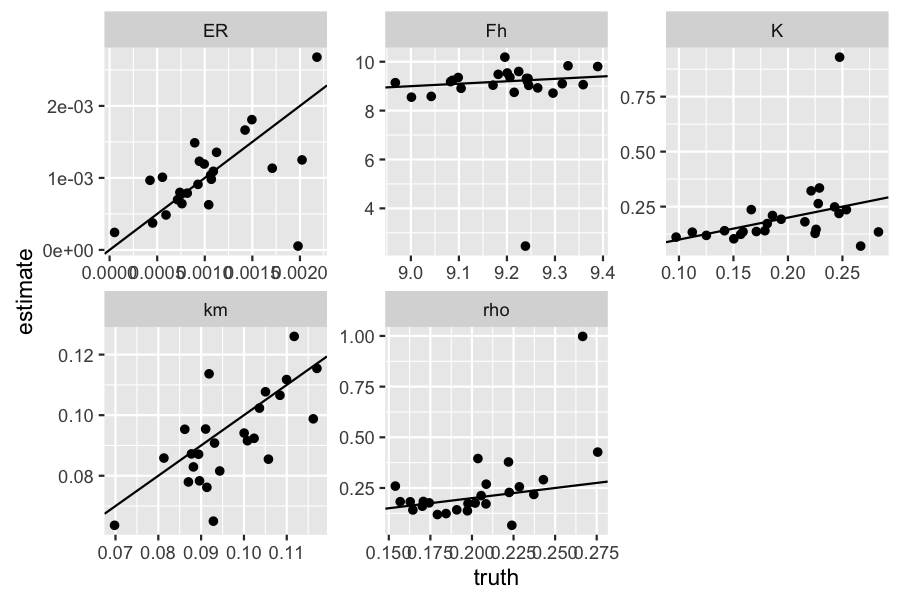
\includegraphics[width=\linewidth]{figure/rep-cost-est-2-1} \hfill{}

\caption[The highest likelihood parameter estimate from fitting each of 25 parameter sets using the model with normal measurement errors]{The highest likelihood parameter estimate from fitting each of 25 parameter sets using the model with normal measurement errors. Note that here I am also estimating the cost of reproduction. The true parameter value is given by the x-axis value and the estimate is given by the y-axis value. The line is the one-to-one line for reference.}\label{fig:rep-cost-est-2}
\end{figure}


\end{knitrout}

Fig. \ref{fig:rel-error-25-2} shows the relative (fractional) error for each parameter, organized by dataset.
Again, these suggest that error was fairly reasonable for most of the datasets.
One of the few datasets that was difficult to estimate was dataset 5.

\begin{knitrout}\scriptsize
\definecolor{shadecolor}{rgb}{0.969, 0.969, 0.969}\color{fgcolor}\begin{figure}

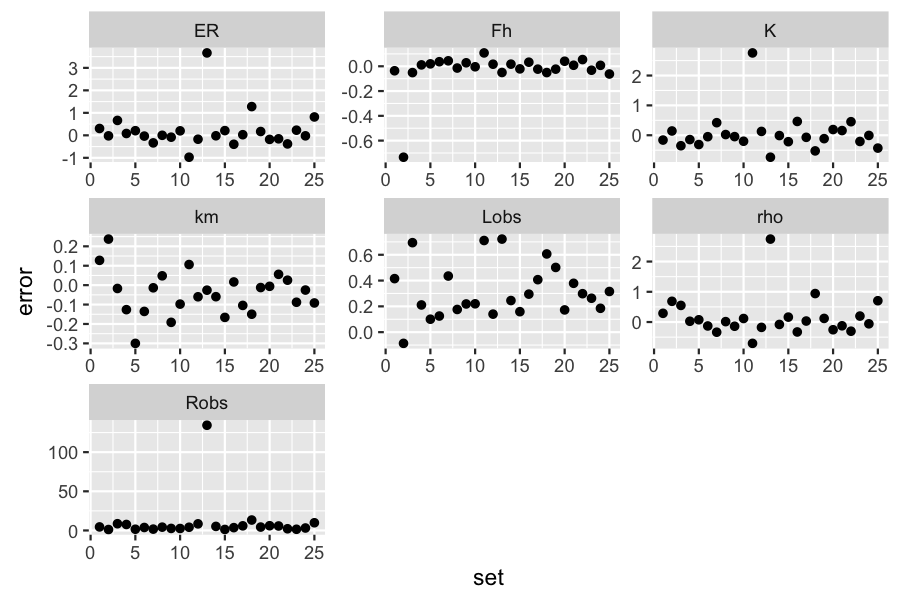
\includegraphics[width=\linewidth]{figure/rel-error-25-2-1} \hfill{}

\caption[Relative error in the parameter estimates for all 25 datasets]{Relative error in the parameter estimates for all 25 datasets.}\label{fig:rel-error-25-2}
\end{figure}


\end{knitrout}

\clearpage

However, if you look at the growth and reproduction trajectories for dataset 5 compared to all of the other growth and reproduction trajectories, you can see that this dataset had the lowest reproduction (the red line in Fig. \ref{fig:comparing-trajectories}).
Another dataset that was somewhat challenging to estimate was dataset 10, which also had low reproduction (the blue line).
Note that the two datasets with very high reproduction were datasets 6 and 19, which have very high estimates of the observation error in reproduction, but the other parameters were well-estimated.

\begin{knitrout}\scriptsize
\definecolor{shadecolor}{rgb}{0.969, 0.969, 0.969}\color{fgcolor}\begin{figure}

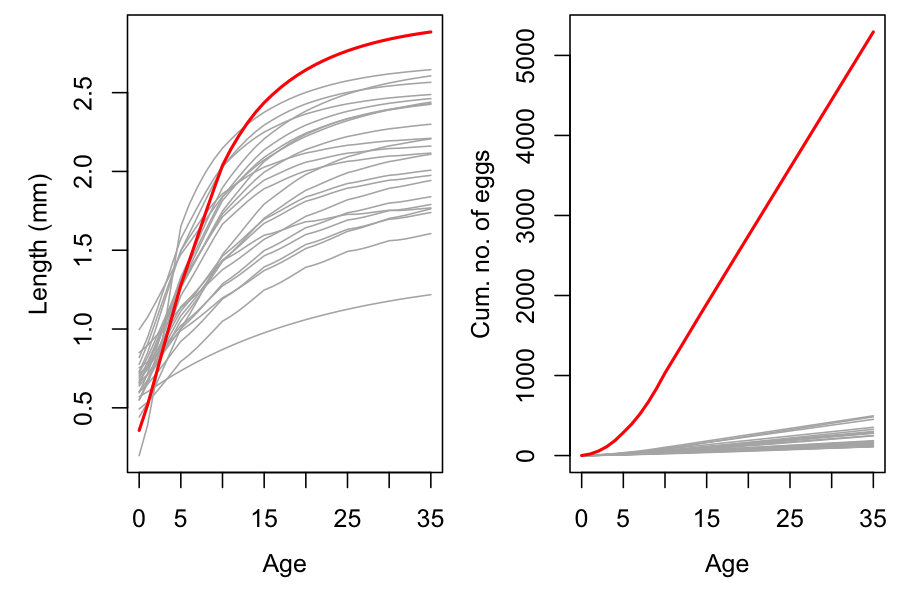
\includegraphics[width=\linewidth]{figure/comparing-trajectories-1} \hfill{}

\caption[The growth and reproduction trajectories at the true parameter values for dataset 13 (black) and all other datasets (grey)]{The growth and reproduction trajectories at the true parameter values for dataset 13 (black) and all other datasets (grey).}\label{fig:comparing-trajectories}
\end{figure}


\end{knitrout}


\clearpage

I am wondering, however, whether I couldn't do better if I increased the size of the initial box of guesses and the number of estimates that I refine through Nelder-Mead.
In particular, I am wondering whether some parameter sets that are somewhat close to the true parameter set have lower likelihoods than other places in parameter space, and are thus excluded from the Nelder-Mead optimization, even though if they were optimized they would end up with higher likelihoods.
Another possibility, of course, is that the true parameter values are actually somewhat less likely than other places and, moreover, sit on a very steep, isolated peak in likelihood space, so that they are hard to find and hard to stay near.
I am going to explore this by initializing optimizations at the true parameter values and then seeing how the results of those optimizations compare with the results from the blind optimization.

Fig. \ref{fig:free-vs-truth-start} shows that, when you start the optimization algorithm at the true parameter values, the ML parameter estimates are closer to the truth (in almost every case) than those started blindly.

\begin{knitrout}\scriptsize
\definecolor{shadecolor}{rgb}{0.969, 0.969, 0.969}\color{fgcolor}\begin{figure}

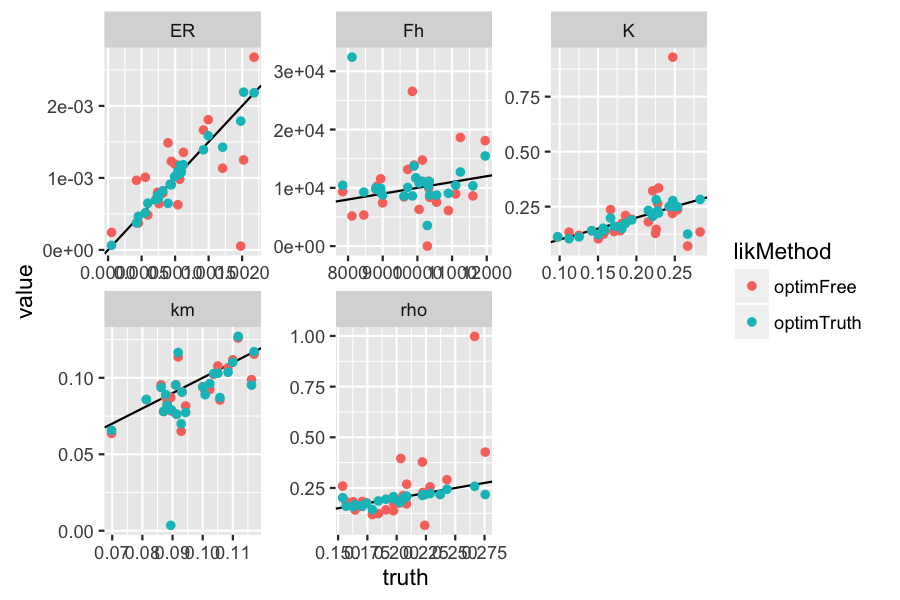
\includegraphics[width=\linewidth]{figure/free-vs-truth-start-1} \hfill{}

\caption[Comparing the true parameter values (x-axis) against the parameter estimates when the optimization algorithm starts from naive guesses and when the algorithm starts at the true parameter values]{Comparing the true parameter values (x-axis) against the parameter estimates when the optimization algorithm starts from naive guesses and when the algorithm starts at the true parameter values.}\label{fig:free-vs-truth-start}
\end{figure}


\end{knitrout}

More interesting, however, are the results of the likelihood calculation.
The likelihoods of the parameter estimates found either by the full optimization process or by starting at the true parameter values are so close that they lie on top of one another for almost every dataset (Fig. \ref{fig:lik-comparison}).
However, the likelihoods of the true parameter sets themselves are always much smaller (i.e., the negative log-likelihood is larger).

\begin{knitrout}\scriptsize
\definecolor{shadecolor}{rgb}{0.969, 0.969, 0.969}\color{fgcolor}\begin{figure}

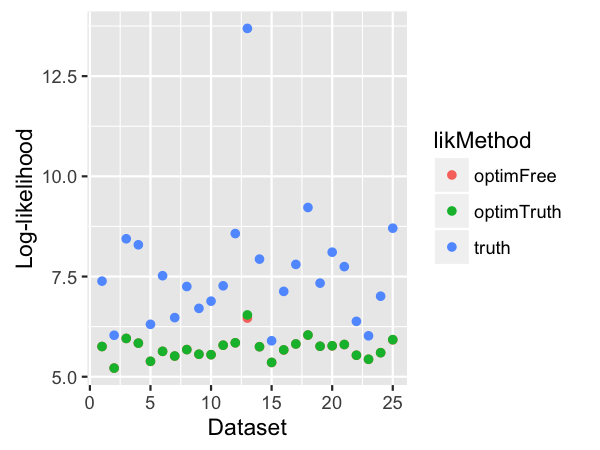
\includegraphics[width=\linewidth]{figure/lik-comparison-1} \hfill{}

\caption[Comparing the likelihood of the true parameter values to the likelihoods obtained by the fitting algorithm when initialized completely randomly and when initialized at the true parameter values]{Comparing the likelihood of the true parameter values to the likelihoods obtained by the fitting algorithm when initialized completely randomly and when initialized at the true parameter values.}\label{fig:lik-comparison}
\end{figure}


\end{knitrout}

\begin{knitrout}\scriptsize
\definecolor{shadecolor}{rgb}{0.969, 0.969, 0.969}\color{fgcolor}\begin{figure}

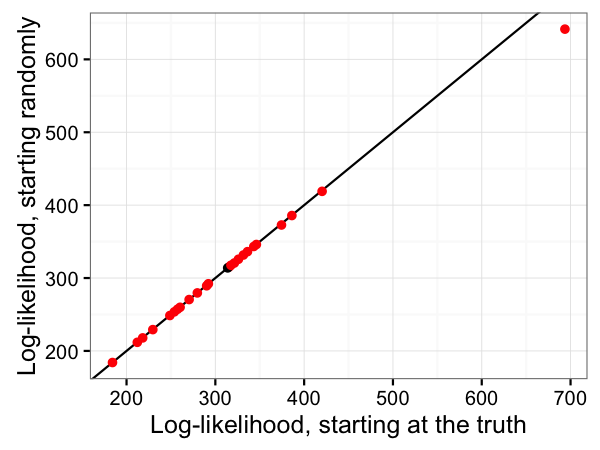
\includegraphics[width=\linewidth]{figure/lik-comparison-2-1} \hfill{}

\caption[Comparing the log-likelihoods found via the optimization algorithm starting without any constraint versus that found from starting at the true parameter values]{Comparing the log-likelihoods found via the optimization algorithm starting without any constraint versus that found from starting at the true parameter values. Red points indicate datasets where the likelihood was lower for the free start.}\label{fig:lik-comparison-2}
\end{figure}


\end{knitrout}

\clearpage

Thus it appears to be generally true that there will be multiple parameter sets that give rise to nearly identical likelihoods, making it impossible to know, in general, which is closer to the truth.
However, the overall message from this fitting is pretty encouraging, as most of the parameter estimates are close to the truth and the algorithm is finding high likelihood parameter sets.
The problem of ridges in likelihood space is almost certain to be unavoidable, but doesn't appear to be completely fatal.


\end{document}
